\documentclass{article}
\usepackage[utf8]{inputenc}

\title{CS 376 : Assignment 6 \\
Modeling and Simulation of Petri Nets}
\author{Fred Eisele }
\date{29 October 2014}

\usepackage{natbib}
\usepackage{graphicx}

\begin{document}

\maketitle

\section{Introduction} \label{sec:intro}
A tourist agency is setting up boat sightseeing tour
where the boats are autonomous vehicles.
You have been employed by the agency to design a control
system that drives the boat along the channels
as described in the following map.


\begin{figure}[h!]
\centering
\includegraphics[scale=0.5]{boat_tour.png}
\caption{Boat Tour}
\label{fig:boat-tour}
\end{figure}

\paragraph
The channel, Figure \ref{fig:boat-tour},
has been divided up into regions.
In the Petri-nets, Figures \ref{fig:pn1}
\ref{fig:pn2} and \ref{fig:pn3}, the places
with names following the pattern $P#$
represent these regions.
The exception to this rule is the $P3A$ and $P3B$
places which represent region #3.
In that case the place represents the path
through the region with $P3A$ representing the
lower path and $P3B$ representing the upper path.
The transitions are named based on the
boundaries between the regions $T##$ where
the first digit is the start region and the
second digit the destination.
A token in any of these places represents a boat.
Tokens in other places represent permision (not boats).


\section{Single Boat Indeterminate Path} \label{sec:1-indet}

Model the problem of a single boat with a Petri net
and describe in detail what each place and transition represents

\begin{figure}[h!]
\centering
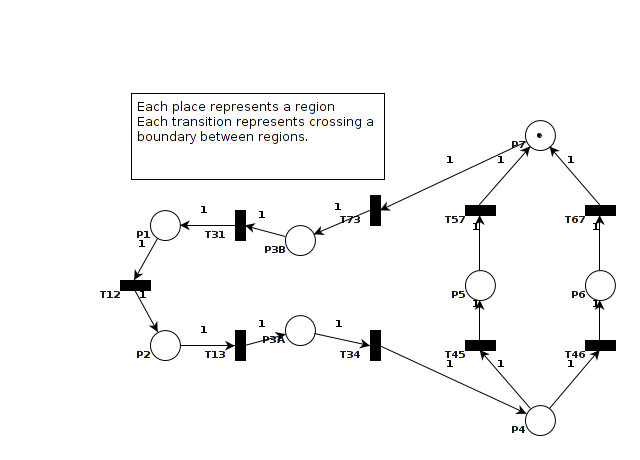
\includegraphics[scale=0.5]{hw6_petri_net_1.png}
\caption{Single Boat with Indeterminate Path}
\label{fig:pn1}
\end{figure}

\paragraph
This produces an indeterminate path as when
there is a token in $P4$ both $T45$ and $T46$ are enabled.

\section{Single Boat Determinate Path} \label{sec:1-det}

The tourist agency wants the
boat to pass alternatively through region 5 and 6.
The Petri net in Section \ref{sec:1-indet} is
modified so that this constraint is satisfied.

\begin{figure}[h!]
\centering
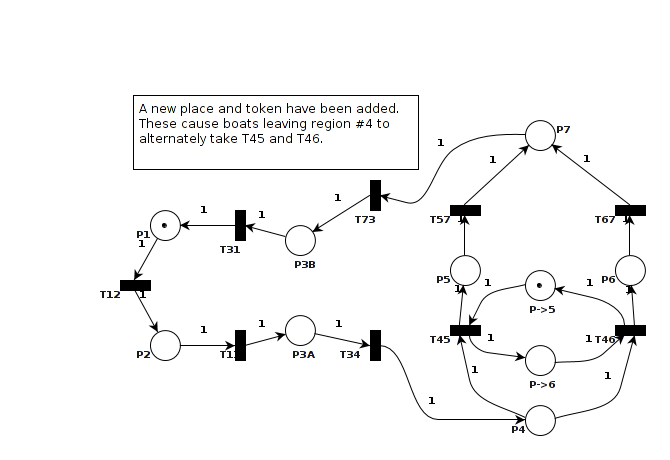
\includegraphics[scale=0.5]{hw6_petri_net_2.png}
\caption{Single Boat with Determinate Path}
\label{fig:pn2}
\end{figure}

This is done by introducing a pair of places,
$P->5$, $P->6$ and a token.
The token acts as a permit for the boat
to enter either $P5$ or $P6$
depending on whether it is in place $P->5$ or $P->6$.


\section{Two Boats Place Exclusion} \label{sec:2-excl}

There are two boats.
This Petri-net models a system like that of
Section \ref{sec:1-det} but it additionally
only allows one boat to access region 3 at a time.

\begin{figure}[h!]
\centering
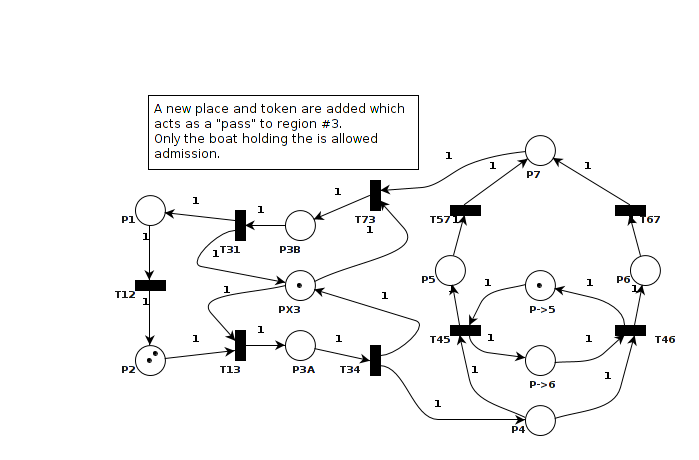
\includegraphics[scale=0.5]{hw6_petri_net_3.png}
\caption{Two Boat with Exclusion Zone and Determinate Path}
\label{fig:pn3}
\end{figure}

\paragraph
This is done by introducing a place,
$PX3$ and a token.
The token acts as a permit for the boat
to enter $P3A$ or $P3B$.
Recall that these two places represent one region.
For this reason the two places compete for the net token.

\end{document}
